\chapter{ACCS Design Challenge ‘ADC 2018’ Showcases Engineering Innovations}

\begin{multicols}{2}

The fifth edition of ACCS Design Challenge (ADC 2018) concluded successfully in the month of March 2019 at the International Institute of Information Technology Bangalore (IIITB). 

ACCS administers the design challenge to provide engineering students, from across the nation, with opportunities for learning beyond curriculum and solve real-life challenges using state-of-the-art technologies. Participating teams developed innovative and effective solutions across application environments in Healthcare, Energy Management, Smart Transportation Systems and Wearable Technologies.  

ADC 2018 was sponsored by M/S Ricoh Innovations Private Limited (RIPL), an R\&D subsidiary of Ricoh Innovations Corporation (RIC), based in Bengaluru. RIPL focuses on delivering advanced smart vision and healthcare solutions. 

Over 150 teams across the country submitted proposals to ADC 2018, which were screened for their uniqueness of concept and innovation. About 95 qualifying teams were invited to present the What, Why and How of their project with the help of a demo, wherever possible, and posters during ADCOM 2018 in September 2018 at Bengaluru. A total of 42 teams advanced to the next round of evaluation in January 2019 and 17 teams competed in the finals for the top honors. 

The finalists showcased their designs with working prototypes, based on NXP's Freedom K64F kits, centred around ARM Cortex M4 series core, provided by Element14. Their designs were reviewed and judged by eminent panel of jurors from across the industry and academia.

The team from SA Engineering College, Chennai, represented by Jagan P, Hariharan VC, Mohamed Ashraf Thaha, and Raghu U, and mentored by Dr. Priya, from the Department of Electrical and Electronics Engineering, won the First Prize for their effort on building a `Bionic arm'.  

\end{multicols}

\begin{figure}[H]
\centering
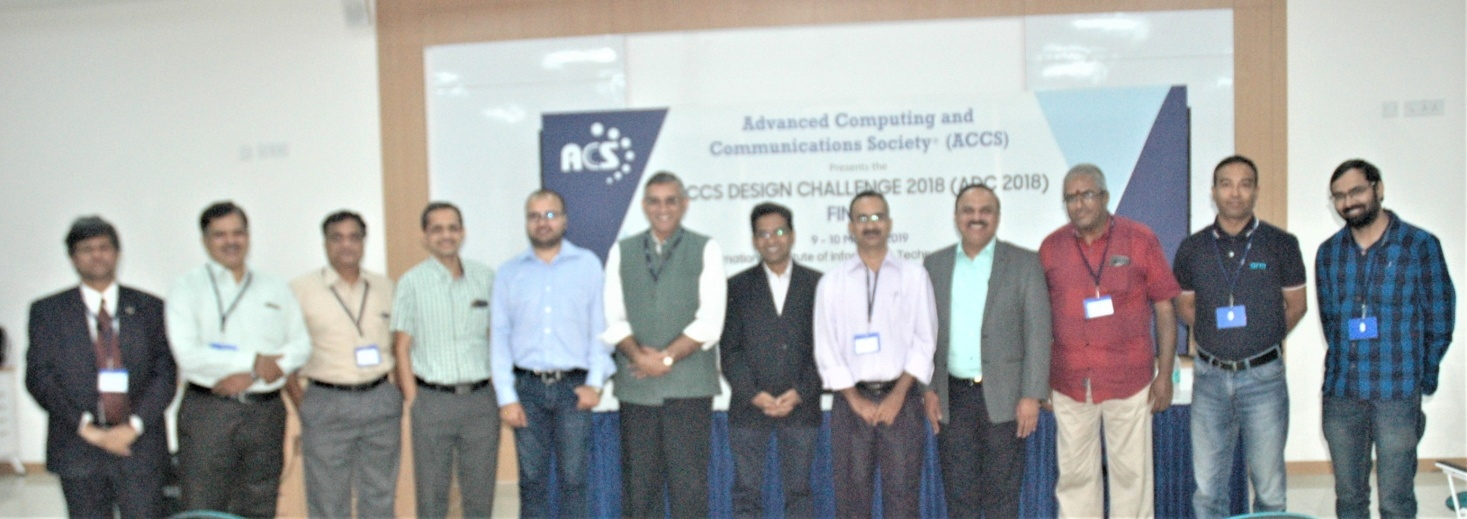
\includegraphics[scale=3.28]{src/Figures/adc.jpg}
\end{figure}


